%\documentclass[german,bachelor]{swsLeipzig}
\documentclass[german,bachelor]{swsLeipzig}
% When you change the language, pdflatex may halt on recompilation.
% Just hit enter to continue and recompile again. This should fix it.

%
% Values
% ------
\ThesisSetTitle{Ermittlung von Konfigurationsoptionen im Source Code mit Fokus auf Machine Learning Bibliotheken in Python}
\ThesisSetKeywords{These, Are, My keywords} % only for PDF meta attributes

\ThesisSetAuthor{Marco Jaeger-Kufel}
\ThesisSetStudentNumber{3731679}
\ThesisSetDateOfBirth{10}{05}{1995}
\ThesisSetPlaceOfBirth{Hannover}

\ThesisSetSupervisors{Prof.\ Dr.\ Norbert Siegmund,Prof.\ Dr.\ Unknown Yet}

\ThesisSetSubmissionDate{14}{06}{2022}

%
% Suggested Packages
% ------------------
\usepackage[sort&compress]{natbib}
%   Allows citing in different ways (e.g., only the authors if you use the
%   citation again within a short time).
%
\usepackage{booktabs}
%    For tables ``looking the right way''.
%
%\usepackage{tabularx}
%    Enables tables with columns that automatically fill the page width.
%
%\usepackage[ruled,algochapter]{algorithm2e}
%    A package for pseudo code algorithms.
%
%\usepackage{amsmath}
%    For tabular-style formatting of mathematical environments.
%

%
% Commenting (by your supervisor)
% -------------------------------
\usepackage{xcolor}
\usepackage{soul}
\usepackage{listings}
\usepackage[euler]{textgreek}
\usepackage{graphicx}
\newcommand{\bscom}[2]{%
  % #1 Original text.
  % #2 Replacement text.
    \st{\scriptsize\,#1}{\color{blue}\scriptsize\,#2}%
  }

% Create links in the pdf document
% Hyperref has some incompatibilities with other packages
% Some other packages must be loaded before, some after hyperref
% Additional options to the hyperref package can be provided in the braces []
\usehyperref[backref] % This will add back references in the bibliography
\usepackage[utf8]{inputenc}
\usepackage{textcomp}
\usepackage{tikz,pgfplots}
\usetikzlibrary{patterns}
\usepackage{float}
\setcitestyle{authoryear,close={)}}

\begin{document}
\begin{frontmatter}
  \begin{abstract}
    A short summary.
  \end{abstract}

  \tableofcontents

  %\chapter*{Acknowledgements} % optional
  %I thank the authors of the swsLeipzig template for their excellent work!

  \listoffigures % optional

  \listoftables % optional

  %\listofalgorithms % optional
  %    requires package algorithm2e

  % optional: list of symbols/notation (e.g., using the nomencl package)
\end{frontmatter}

\chapter{Einleitung}\label{Einleitung}
%Diese Arbeit entsteht am Institut für Informatik an der Universit\"at Leipzig in der Abteilung \glqq Softwaresysteme\grqq.
%Im Folgenden wird die zugrundeliegende Problemstellung und Relevanz erl\"autert.
%Anschlie\ss end wird dieses Problem auf einen konkreten Anwendungsbereich \"ubertragen und auf die Zielsetzung der Arbeit eingegangen.\\

\section{Motivation}
Moderne Softwaresysteme erm\"oglichen den Nutzenden ein breites Spektrum unterschiedlicher Konfigurationsoptionen.
Anhand dieser Konfigurationsoptionen sind die Nutzenden in der Lage, viele Aspekte der Ausgestaltung einer Software zu steuern.
Konfigurationsoptionen k\"onnen dabei ganz unterschiedliche Funktionen besitzen, die von den Nutzenden nach den eigenen Bed\"urfnissen angepasst werden k\"onnen.\\

Konfigurationsoptionen können in verschiedenen Teilen eines Softwareprojekts verarbeitet, definiert und beschrieben werden:
in der Konfigurationsdatei, im Source Code und in der Dokumentation \cite[S. 185]{7774519}.
Sie werden meist als Key-Value Pair entworfen und gesammelt in einer Konfigurationsdatei gespeichert.
Dem Namen der Konfigurationsoption (Key) werden dabei Einstellungsmöglichkeiten beliebigen Typs zugeordnet (Value).
Zur Speicherung von Konfigurationsoptionen verwenden einige Systeme, wie das Big Data-Framework Hadoop, strukturierte XML-Formate oder auch JSON-Dateien.
Ein einheitliches Schema zur Speicherung als Konfigurationsdatei gibt es jedoch nicht, weshalb sich diese von der Struktur und Syntax unterscheiden. \cite[S. 131]{10.1145/1985793.1985812}.
Im Source Code können die Konfigurationsoptionen eingelesen und bearbeitet werden \cite[S. 185]{7774519}.\\

W\"ahrend die Vielf\"altigkeit und Individualisierbarkeit der Software gr\"o\ss er wird, erh\"oht sich auch die Komplexit\"at der Software f\"ur Entwickler und Entwicklerinnen.
Vor allem das Warten und Testen der Konfigurationsmöglichkeiten gestaltet sich nun umfangreicher.
Besonders problematisch wird es, wenn Konfigurationsoptionen auf unvorhergesehene Weise interagieren.
Solche Abh\"angigkeiten sind in einem wachsenden Spielraum m\"oglicher Kombinationen schwer zu entdecken und zu verstehen.
Entwickler und Entwicklerinnen m\"ussen die Konfigurationsoptionen innerhalb der Software verfolgen, um festzustellen,
welche Codefragmente von einer Option betroffen sind und wo und wie sie mit ihr interagieren.
Des Weiteren kann es vorkommen, dass Entwickler und Entwicklerinnen Werte von Konfigurationsoptionen nicht aktualisieren, was dazu führen kann,
dass über mehrere Module hinweg, unbemerkt mit falschen Werten gearbeitet wird \cite[S. 185]{7774519}.
Die verschiedenen m\"oglichen Auspr\"agungen einer Konfigurationsoption erschweren hierbei die Nachvollziehbarkeit des Kontrollflusses der Software.\\

In einer empirischen Studie über Konfigurationsfehler stellen \citeauthor{10.1145/2043556.2043572} (\citeyear{10.1145/2043556.2043572}, S. 160) fest,
dass in kommerziellen Softwareunternehmen für Speicherlösungen, knapp ein Drittel aller Ursachen von Kundenproblemen auf Konfigurationsfehler zurückzuführen sind (siehe Tabelle 3).
Bei Konfigurationsfehler sind Source Code und die Eingabe zwar korrekt, es wird jedoch ein falscher Wert für eine Konfigurationsoption verwendet,
sodass sich die Software nicht wie gewünscht verhält \cite[S. 152]{10.1145/2568225.2568251}.
Solche Fehler können dazu führen, dass die Software abstürzt, eine fehlerhafte Ausgabe erzeugt oder nur unzureichend funktioniert \cite[S. 152]{10.1145/2568225.2568251}.\\

Konfigurationsfehler entstehen zum Beispiel durch die Verwendung unterschiedlicher Versionen einer Software.
Im folgendem Codeausschnitt wird die Klasse \textit{LogisticRegression} der Machine Learning-Bibliothek \textit{scikit-learn} initialisiert und der Variable \textit{clf} zugewiesen:\\

\begin{lstlisting}[language=Python, frame=single]
from sklearn.linear_model import LogisticRegression
clf = LogisticRegression()
\end{lstlisting}
\

Da keine Parameter angegeben werden, wird die Klasse mit den Default-Werten initialisiert, zum Beispiel
\textit{max\_iter = 100, verbose = 0, n\_jobs = 1}.
In der Version \textit{scikit-learn 0.21.3} wird für den Parameter \textit{multi\_class} als Default noch der Wert \textit{ovr} zugewiesen (\citeyear{sklearn}).
Für alle nachfolgenden Versionen ist der Default-Wert für diesen Parameter jedoch \textit{auto} (\citeyear{sklearn}).
Folglich führt die Verwendung dieser Klasse ohne explizite Parameterangabe, nach Verwendung unterschiedlicher Versionen, zu schwer nachvollziehbaren Programmverhalten.\\

Bei den Parametern eines solchen Machine Learning Algorithmus, die vor Beginn des Lernprozesses vom Nutzenden festgelegt werden können,
spricht man dabei von sogenannten \textit{Hyperparametern}.
Sie werden als Parameter an die jeweilige Klasse übergeben und bieten den Nutzenden Konfigurationsmöglichkeiten für
das Training des Modells.
In dem obigen Fall können so beispielsweise über den Parameter \textit{max\_iter} die Anzahl der Trainingsiterationen
der Logistischen Regression festgelegt werden und über \textit{n\_jobs} die maximale Anzahl der parallel zu verwendenden CPU-Kernen.
Durch das Extrahieren dieser Konfigurationswerte, können die Parameter statisch geprüft werden, was für den Nutzenden
eine Zeitersparnis bedeutet, wenn sonst ein falscher Konfigurationswert einen langen Batch-Job zum Scheitern bringt
oder das Ergebnis nicht den Erwartungen entspricht. \\



\section{Anwendungsbereich und Zielsetzung}
Das Ziel dieser Arbeit ist es, Konfigurationsoptionen im Source Code zu erkennen und zu extrahieren. \\

Es existieren bereits einige Forschungsansätze zur Ermittlung und Verarbeitung von Konfigurationsoptionen im Source Code.
Viel zitiert wird dabei der Ansatz von \citeauthor{10.1145/1985793.1985812}, den sie \citeyear{10.1145/1985793.1985812} publizierten.
Wie auch \citeauthor{7774519} oder \citeauthor{8049300} entwickelten sie einen Ansatz, mittels statischer Code-Analyse Konfigurationsoptionen
im Source Code zu tracken.
Dabei fokussierten sie sich auf die Programmiersprache Java, die nach dem TIOBE-Index jahrelang als beliebteste Programmiersprache galt (\citeyear{enwiki:1077809155}).
Der TIOBE-Index misst die Popularität von Programmiersprachen auf der Grundlage von Suchanfragen auf beliebten Websites und in Suchmaschinen (\citeyear{enwiki:1077809155}).
Im Februar 2022 ist in diesem Ranking Python erstmals zur beliebtesten Programmiersprache aufgestiegen (\citeyear{enwiki:1077809155}).
Für Python ist diese Thematik jedoch bislang allerdings noch wenig beleuchtet. \\

Die Programmiersprache Python ist für ihre Benutzendenfreundlichkeit bekannt und obwohl Python eine interpretierte High-Level-Programmiersprache ist,
ist sie in der Lage, bei Bedarf die Leistung von Programmiersprachen auf Systemebene zu nutzen \cite[S. 2]{2020}.
Insbesondere im Bereich wissenschaftliches Rechnen (Scientific Computing) gewann Python in den letzten Jahren enorm an Popularität,
weshalb viele Bibliotheken für maschinelles Lernen auf Python basieren \cite[S. 2]{2020}. \\

Gegenstand dieser Arbeit werden daher Konfigurationsoptionen sein, die in Python Source Code vorliegen und mittels statischer Code-Analyse erkannt werden.
Der Ansatz identifiziert automatisch die Stellen im Source Code, an denen die Optionen der zu untersuchenden Bibliotheken gelesen werden
und ermittelt für jede dieser Stellen den Namen der Option.
Darauf aufbauend erfolgt eine Datenflussanalyse, um auch für Optionen, die in Form von Variablen als Parameter übergeben werden,
die möglichen Werte zu ermitteln.
Der Fokus auf drei der populärsten Machine Learning Bibliotheken in Python (siehe \autoref{fig:kaggle}):
\begin{itemize}
 \item TensorFlow
 \item PyTorch
 \item scikit-learn
\end{itemize}
Zudem wird die Verwendung von Konfigurationsoptionen der Machine Learning Lifecylce Plattform \textit{MLflow} untersucht. \\


\section{Aufbau dieser Arbeit und methodisches Vorgehen}
% Umsetzung gleidert isch in 3 Schritte: WEbscrping, nochmal auf Klassen eingehen, Statische Code-Analyse mit ReadPoint, und extrahieren der Parameter,
% Am Ende einfpelgen in s Cg net

\chapter{Hintergrund}\label{Hintergrund}

\section{Statische Code-Analyse}
Das wichtigste Werkzeug dieser Arbeit ist die statische Code-Analyse,
mit der Software-Projekte unabhängig von der Ausführungsumgebung untersucht werden können.
Die statische Code-Analyse ist ein Werkzeug, um Fehler in einer Softwareanwendung zu reduzieren \cite[S. 99]{bardas2010static}.
So ermöglichen sie den Anwendenden, Fehler in einem Programm zu finden, die für den Compiler nicht sichtbar sind \cite[S. 99]{bardas2010static}.\\

Im Gegensatz zur dynamischen Analyse wird die statische Analyse zur Übersetzungszeit durchgeführt
und setzt damit bereits vor der tatsächlichen Ausführung des Source Codes an \cite[S. 2]{gomes2009overview}.
Die erzeugten Ergebnisse der statischen Analyse lassen sich besser Verallgemeinern, da sie nicht abhängig von den Eingaben sind,
mit denen das Programm während der dynamischen Analyse ausgeführt wurde \cite[S. 6]{gomes2009overview}.\\

Für das Aufspüren von Konfigurationsoptionen bietet sich eine statische Code-Analyse daher aus mehreren Gründen an.
So kann es viele Optionen geben, die nur in bestimmten Modulen oder als Folge bestimmter Eingaben verwendet werden.
%Es ist unwahrscheinlich, dass mittels dynamischen Testens alle Verwendungen der gesuchten Konfigurationsoptionen gefunden werden.
%Dies würde zudem bei größeren Softwareprojekten eine sehr komplexe Test-Suite erfordern, um möglichst alle Fälle abdecken zu können.
Mit der statischen Code-Analyse kann eine hohe Abdeckung hingegen deutlich leichter erreicht werden.
Gleichzeitig verbergen sich hinter den Methoden und Klassen, der zu untersuchenden Machine Learning Bibliotheken,
teils sehr komplexe und rechenintensive Berechnungen, die bis zu mehrere Tage laufen könnten.
Aus Kosten-Nutzen-Gründen ist hier eine dynamische Analyse nur bedingt sinnvoll.\\

\section{Datenflussanalyse}
Die Datenflussanalyse ist ein Werkzeug, um Informationen über die möglichen Werte, die an verschiedenen
Stellen in einem Codesegment berechnet werden, zu erfassen \cite[S. 1537]{58766}.
Es handelt sich um eine statische Analysetechnik mit dem Ziel, das Programmverhalten schon zur Übersetzungszeit,
also bevor es ausgeführt wurde, zu bestimmen.
Der Datenfluss kann mittels eines Kontrollflussgraphens dargestellt werden und dem Betrachtenden
Rückschlüsse über das Verhalten des Programms geben.
Der Graph zeigt an, an welchen Stellen eine Variable verwendet wird und welche Werte sie annehmen kann.\\

Es gibt verschiedene Techniken, die innerhalb der Datenflussanalyse eingesetzt werden, um den Wert von Variablen zu bestimmen.
Eine von ihnen ist \textit{Constant Propagation}.
Das Ziel von Constant Propagation ist zu bestimmen, an welchen Stellen im Programm, eine Variable einen konstanten Wert besitzt.
So kann zum Beispiel toter Code, also redundanter Code, der im weiteren Programmverlauf nicht weiter verarbeitet wird, gefunden werden.\\

Eine weitere Technik ist \textit{Static Single Assignment}.
Bei dieser Methodik werden die Variablen im Verlauf des Übersetzungsprozesses in eine Zwischenform überführt, in der jede Variable
genau einmal zugewiesen wird.
Die Variablen werden in Versionen aufgeteilt und in der Regel mit einem aufsteigendem Index versehen,
sodass jede Definition ihre eigene Version erhält.\\

Die beide Techniken Static Single Assignment und Constant Propagation werden in dem statischen Analyse-Framework
\textit{Scalpel} kombiniert.
Aus dem folgenden Codebeispiel geht hervor, dass die Variable \textit{a} zwei unterschiedliche Werte annehmen kann.\\

\begin{lstlisting}[language=Python, frame=single]
c = 10
a = -1
if c > 0:
    a = a + 1
else:
    a = 0
total = c + a
\end{lstlisting}
\

Der daraus resultierende Kontrollflussgraph besteht charakteristisch aus Knoten, die die jeweilige Code-Objekte beinhalten und gerichtete Kanten als Übergang
zwischen den Knoten, die den Programmablauf darstellen.
Mittels Constant Propagation werden die tatsächlichen Werte der Variablen an den jeweiligen Verwendungszeitpunkten erkannt
und über die \textPhi-Funktion kann durch Static Single Assignment abgeleitet werden, dass es zwei mögliche Rückgabewerte gibt.

\begin{figure}[h]
 \centering
 \includegraphics[scale=0.8]{ssa_diagram}
 \caption{Kontrollflussgraph \cite[]{li2022scalpel}}
 \label{fig:scalpel}
\end{figure}


\section{Maschinelles Lernen}
Die künstliche Intelligenz (KI) ist ein Teilgebiet der Informatik und befasst sich mit der Entwicklung von Computerprogrammen und Maschinen,
die in der Lage sind, Aufgaben auszuführen, die Menschen von Natur aus gut beherrschen \cite[S. 1]{2020}.
Dazu gehören zum Beispiel die Verarbeitung von natürlicher Sprache (Natural Language Processing) oder Bilderkennung (Computer Vision).
In der Mitte des 20. Jahrhunderts entstand das maschinelle Lernen (ML) als Teilbereich der KI und schlug eine neue Richtung
für die Entwicklung von künstlicher Intelligenz ein, inspiriert vom konzeptionellen Verständnis der Funktionsweise des menschlichen Gehirns \cite[S. 1]{2020}.\\

Pionier Arthur Samuel definiert maschinelles Lernen als ein Fachgebiet, das Computern die Fähigkeit verleiht, zu lernen,
ohne ausdrücklich programmiert zu werden \cite[S. 381]{mahesh2020machine}.
Es befasst sich mit der wissenschaftlichen Untersuchung von Algorithmen und statistischen Modellen,
die Computersysteme verwenden, um eine Aufgabe zu lösen \cite[S. 381]{mahesh2020machine}.
Dabei werden statistische Methoden verwendet, um aus Daten zu lernen und Muster zu erkennen. \\

%Maschinelles Lernen (ML) wird eingesetzt, um Maschinen beizubringen, wie sie Daten effizienter verarbeiten können.
%Manchmal können wir nach der Sichtung der Daten die Informationen, die wir aus den Daten gewinnen, nicht interpretieren.
%In diesem Fall wenden wir maschinelles Lernen an.
%Mit der Fülle der verfügbaren Datensätze steigt auch die Nachfrage nach maschinellem Lernen.
%Viele Branchen setzen maschinelles Lernen ein, um relevante Daten zu extrahieren.
%Der Zweck des maschinellen Lernens besteht darin, aus den Daten zu lernen.
%Es wurden viele Studien darüber durchgeführt, wie Maschinen selbständig lernen können, ohne explizit programmiert zu werden.
%Viele Mathematiker und Programmierer wenden verschiedene Ansätze an, um eine Lösung für dieses Problem zu finden, das riesige Datensätze umfasst.

\subsection{Ursprung}
Der Ursprung des maschinellen Lernens liegt bereits in der Mitte des 20. Jahrhunderts, als der Psychologoe Frank Rosenblatt
von seiner Arbeitsgruppe eine Maschine zur Erkennung von Buchstaben des Alphabets bauen ließ \cite[S. 1385]{FRADKOV20201385}.
Das Konzept der Maschine basiert auf der Verarbeitung von Signalen analog zum menschliche Nervensystem, weshalb sie
als Prototyp der modernen künstlichen neuronalen Netze gilt \cite[S. 1385]{FRADKOV20201385}.
Der kommerzielle Durchbruch ließ dennoch bis auf den Anfang des 21. Jahrhunderts auf sich warten.
Nach \citeauthor{FRADKOV20201385} ist dies auf drei Trends zurückzuführen, die zusammen einen spürbaren Synergieeffekt bewirkten \cite[S. 1387]{FRADKOV20201385}. \\

Unter anderem durch den Erfolg und Möglichkeiten des Internets ist nicht nur das Vorhandensein von Daten enorm gewachsen,
auch ihre Heterogenität führt dazu, dass herkömmliche Methode zur Verarbeitung und Informationsgewinnung nicht mehr ausreichen \cite[S. 1387]{FRADKOV20201385}.
Durch das Aufkommen von \textit{Big Data} werden neue Ansätze des maschinellen Lernens nicht nur aus dem Motiv des wissenschaftlichen Erkenntnisgewinns entwickelt,
sondern auch aufgrund der praktischen und kommerziellen Notwendigkeit, die rasant wachsenden generierten Datenmengen leistungsfähig verarbeiten zu können. \\

Ein weiterer entscheidender Faktor ist die Senkung der Kosten für parallele Berechnung und Speicher.
Dies umfasst die Weiterentwicklung und Verwendung von Grafikprozessoren (vor allem von Nvidia),
die zu erheblichen Verbesserungen der Rechenleistung führen \cite[S. 1387]{FRADKOV20201385}.
Gleichzeitig sinken die Kosten für Arbeitsspeicher stetig, was die Verarbeitung großer Datenmengen zusätzlich erleichtert \cite[S. 1387]{FRADKOV20201385}.
Aus Softwaresicht kommt schließlich die MapReduce-Technologie von Google bzw. später auch Hadoop hinzu, die es ermöglicht,
komplexe Berechnungen auf mehrere Prozessoren zu verteilen\cite[S. 1387]{FRADKOV20201385}. \\

Der dritte Trend ist die Entwicklung künstlicher neuronaler Netze, die um ein Vielzahl an Zwischenschichten erweitert wurden
und so noch komplexere Berechnungen ausführen können.
In diesem Zusammenhang spricht man auch von \textit{Deep Learning}. \\

\subsection{Algorithmische Ansätze}
Im Allgemeinen werden die Ansätze des maschinellen Lernens in drei große Kategorien unterteilt, je nach Art des \textit{Signals}
oder \textit{Feedbacks}, das dem lernenden System zur Verfügung steht \cite[S. 2]{FRADKOV20201385}:
\begin{itemize}
 \item Überwachtes Lernen (supervised learning)
 \item Unüberwachtes Lernen (unsupervised learning)
 \item Bestärkendes Lernen (reinforcement learning)
\end{itemize}

Das \textit{überwachte Lernen} erfordert ein Training mit gelabelten Daten, die Eingaben und gewünschte Ausgaben haben \cite[S. 2]{cite-key}.
So weiß das Modell zum Beispiel, ob auf einem bestimmten Foto ein Hund abgebildet ist oder wie viel ein bestimmtes Haus kostet.
Auf dieser Grundlage kann es dann so trainiert werden, dass es neue Hunde erkennt oder den Preis neuer Häuser schätzt. \\

Im Gegensatz dazu erfordert das \textit{unüberwachte Lernen} keine markierten Trainingsdaten und erhält lediglich Eingabedaten \cite[S. 2]{cite-key}.
Die richtige Antwort ist entweder nicht bekannt oder existiert nicht.
Stattdessen sucht das Modell nach sinnvollen Strukturen in den Daten, um neue Erkenntnisse über ein Thema zu gewinnen \cite[S. 383]{mahesh2020machine}.
Unüberwachtes Lernen kann zum Beispiel dazu verwendet werden, in einem Online-Store Kunden zu finden, die einen ähnlichen Geschmack haben,
und Artikel empfehlen, die diese Kunden gekauft haben. \\

Das \textit{bestärkende Lernen} hingegen unterscheidet sich sehr deutlich von den beiden vorherigen Kategorien.
Das Modell ist hier ein aktiver Akteur, das mit seiner externen Umgebung interagiert
und positives oder negatives Feedback für seine Handlungen erhält \cite[S. 2]{cite-key}.
Aus diesen Rückmeldungen erlernt es optimale Handlungsstrategien für seine Umgebung zu entwickeln \cite[S. 384]{mahesh2020machine}.
Solche Modelle können zum Beispiel für selbstfahrende Autos verwendet werden oder um einer Maschine Gesellschaftsspiele beizubringen.\\

\subsection{Python-Bibliotheken}
Fürs maschinelle Lernen gilt Python schon seit langem als erste Wahl für Entwickler und Entwicklerinnen.
Eine im Mai \citeyear{nugget} veröffentlichte Umfrage vom Portal \citeauthor{nugget} ergab, dass Python in der Kategorie
\glqq Top Analytics, Data Science, Machine Learning Tools\grqq{} von rund 66\% der Teilnehmenden verwendet wird
und damit die populärste Programmiersprache in diesem Bereich ist \cite{nugget}. \\

Python ist eine interpretierte Programmiersprache.
Demnach wird während der Ausführung der Python-Code zur Laufzeit interpretiert, wodurch sie im Vergleich mit kompilierten
Programmiersprachen wie C / C++ hinsichtlich Leistung und Geschwindigkeit schlechter abschneidet.
Ein wichtiger Vorteil von Python ist jedoch die Möglichkeit, Code aus anderen Programmiersprachen relativ einfach einzubinden \cite[S.977]{8757088}.
Viele Lösungen im maschinellen Lernen basieren auf numerischen und vektorisierten Berechnungen mit Bibliotheken
wie \textit{NumPy} oder \textit{SciPy} \cite[S.977]{8757088}.
Um diese Berechnungen schnell und effizient auszuführen, werden sogenannte \textit{Wrapper} verwendet,
die Algorithmen von kompilierten Programmiersprachen implementieren \cite[S.977]{8757088}.
Die wahrscheinlich am häufigsten verwendete Bibliothek für diesen Zweck ist Cython, die zwar auf Python basiert,
aber auch den Aufruf von Funktionen, sowie die Verwendung von Variablen und Klassen aus der Programmiersprache C unterstützt \cite[S.977]{8757088}.
Dadurch können kritische Teile des Codes um ein Vielfaches beschleunigt werden. \\

Einer der Hauptgründe für die Populärität von Python ist das riesige Ökosystem, das aus einer Vielzahl
von umfangreichen und leistungsfähigen Bibliotheken besteht, über die eben angesprochene Algorithmen aufgerufen werden können,
wodurch die Benutzendenfreundlichkeit bei gleichzeitiger Effizienz in der Performanz gewahrt bleiben kann \cite[S. 2]{2020}.
So sind nach einer jährlich von der Data Science-Plattform \citeauthor{kaggle} durchgeführten Umfrage unter rund 25.000 ML-Engineers
und Data Scientists, die Python Bibliotheken mit großem Abstand die am meisten genutzten Frameworks für maschinelles Lernen \cite[]{kaggle}.

\begin{figure}[H]
\begin{center}
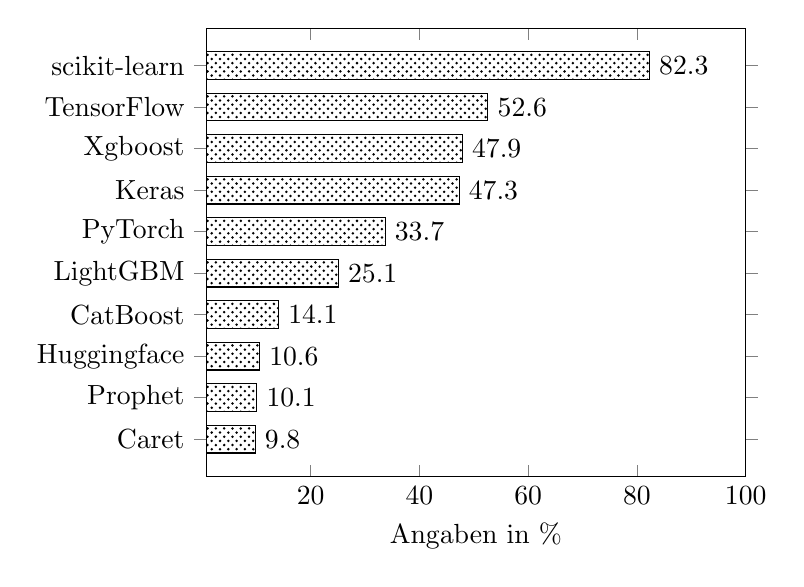
\begin{tikzpicture}
    \begin{axis}[
        xbar,
        xmax=100,
        nodes near coords,
        xlabel={Angaben in \%},
        symbolic y coords={Caret,Prophet,Huggingface,CatBoost,LightGBM,PyTorch,Keras,Xgboost,TensorFlow,scikit-learn},
        ytick = data,
  ]
  \addplot [pattern=crosshatch dots,pattern color=black] coordinates { (82.3,scikit-learn)(52.6,TensorFlow)(47.9,Xgboost)(47.3,Keras)(33.7,PyTorch)(25.1,LightGBM)(14.1,CatBoost)(10.6,Huggingface)(10.1,Prophet)(9.8,Caret)};
  \end{axis}
\end{tikzpicture}
\caption{Nutzung von ML-Frameworks \cite[]{kaggle}} \label{fig:kaggle}
\end{center}
\end{figure}

Aus der Grafik lassen sich drei der zu untersuchenden Python Bibliotheken entnehmen.
Zum einen \textit{scikit-learn}, das aufgrund der Vielzahl an implementierten Algorithmen wie ein \glqq schweizer Taschenmesser\grqq{}
für die meisten Projekte eingesetzt werden kann und von über 80\% der Befragten verwendet wird \cite[]{kaggle}.
Die Vorteile von scikit-learn ist die benutzerfreundliche Struktur und Dokumentation mit der maschinelles Lernen
auch für unerfahrene oder fachfremde Menschen zugänglich gemacht wird \cite[S.29]{10.1145/2786984.2786995}.\\

Bei der zweiten zu untersuchenden Bibliothek handelt es sich um \textit{TensorFlow}.
Nachdem es 2015 von Forschern bei Google ursprünglich für interne Zwecke entwickelt wurde, hat sich TensorFlow vor allem im Bereich
Deep Learning als populäres Werkzeug bewährt \cite[S. 227]{doi:10.3102/1076998619872761}.
So bietet TensorFlow Projekte, die viel Customizing erfordern, eine leistungsfähige und flexible Umgebung, die das Trainieren
künstlicher neuronaler Netze vereinfacht und beschleunigt \cite[S. 227]{doi:10.3102/1076998619872761}.\\

Die dritte zu untersuchende Bibliothek \textit{PyTorch} wird zwar insgesamt weniger häufig verwendet, verzeichnet
jedoch Jahr für Jahr ein starkes Wachstum in der Nutzung \cite[]{kaggle}.
PyTorch ist vor allem nützlich beim Umgang mit künstlichen neuronalen Netzen, weshalb es 2019 auch die
meistgenutzte Deep Learning-Bibliothek auf allen großen Deep Learning-Konferenzen war \cite[S. 23]{2020}.\\

\textit{MLflow} ist wie die eben aufgeführten Bibliotheken Open Source und wurde vom Silicon Valley Startup databricks 2018 ins Leben gerufen \cite[S. 39]{zaharia2018accelerating}.
Ziel der Plattform ist dabei den Lebenszyklus von ML-Projekten ganzheitlich zu strukturieren \cite[S. 39]{zaharia2018accelerating}.
Dabei werden über die ML-Algorithmen hinaus, den Anwendenden Werkzeuge mit in die Hand zu geben, um den Herausforderungen
von ML-Projekten gegenüber herkömmlicher Softwareentwicklungsprozesse zu begegnen \cite[S. 44]{zaharia2018accelerating}.\\


\subsection{Konfigurationsoptionen}
In objektorientierten Programmiersprachen wie Python sind Klassen einer der grundlegenden Bausteine, die bei der Entwicklung und Anwendung
von maschinellem Lernen eingesetzt werden.
Sie bieten die Möglichkeit, Daten und Funktionen zu kombinieren und dem Nutzenden von Machine Learning Bibliotheken,
bereits vorformulierte Algorithmen aufzurufen.
Dabei werden die Konfigurationsoptionen beim Aufruf der jeweiligen Klasse als Parameter übergeben, sodass die Algorithmen
an die Bedürfnisse des Anwendenen angepasst werden können.
So kann die zielgerichtete Nutzung effizienter und komplexer Algorithmen bei gleichzeitiger Konfigurierbarkeit gewährleistet werden. \\

Bei den Konfigurationsparametern von Lernalgorithmen handelt es sich um sogenannte \textit{Hyperparameter}.
Lernalgorithmen ermöglichen einem Computerprogramm den menschlichen Lernprozess mittels statistischer Methoden zu imitieren.
Sie werden zur Mustererkennung, Klassifizierung und Vorhersage verwendet, indem sie aus einem vorhandenen Trainingsdatensatz
lernen.
Hyperparameter werden festgelegt bevor der Lernprozess beginnt und um den Lernprozess zu steuern \cite[S. 280]{hype}.
Da sich die Algorithmen oft sehr unterschiedlich verhalten, wenn sie mit verschiedenen Hyperparameter instanziiert werden,
wurden in den letzten Jahren eine Vielzahl an Hyperparameter-Optimierungsverfahren entwickelt \cite[S. 1]{pmlr-v32-hutter14}.
Optimierte Hyperparameter können die Leistungsfähigkeit eines Modells oder die Geschwindigkeit und Qualität Lernprozesses stark beeinflussen \cite[S. 280]{hype}.\\

Im folgenden Codebeispiel wird der \textit{Gradient Boosting Classifier} aus der scikit-learn Bibliothek betrachtet.\\

\begin{minipage}{\linewidth}
\begin{lstlisting}[language=Python, frame=single]
from sklearn.ensemble import GradientBoostingClassifier

gbc = GradientBoostingClassifier(n_estimators=20,
        learning_rate=0.05, max_features=2, max_depth=2,
        random_state=0)
\end{lstlisting}
\end{minipage}
\

Es wird eine Instanz dieser Klasse erzeugt und der Variable \textit{gbc} zugewiesen.
Die Klasse verfügt über 20 Parameter (Version 1.0.2), die, sofern bei der Instanziierung für den jeweiligen Parameter
kein neuer Wert zugewiesen wird, mit einem eigenen Default-Wert initialisiert werden.
So werden im Beispiel, den Hyperparametern wie \textit{n\_estimators}, \textit{learning\_rate} oder \textit{max\_depth}
Zahlenwerte übergeben, die von den Default-Werten abweichen.\\


\section{Web Scraping}
Web Scraping ist eine Technik, um Daten aus dem World Wide Web zu extrahieren, um sie später abrufen oder analysieren zu können \cite[S. 1]{zhao2017web}.
Dafür werden die Webdaten über das Hypertext Transfer Protocol (HTTP) oder über einen Webbrowser ausgelesen \cite[S. 1]{zhao2017web}.
Dies kann entweder manuell durch den jeweiligen Benutzenden oder automatisch durch einen Bot oder Webcrawler erfolgen \cite[S. 1]{zhao2017web}.
Ein Web Scraper simuliert das menschliche Browsing-Verhalten im Web, um aus verschiedenen Websites
detaillierte Informationen in einer vorgegebenen Struktur zu sammeln \cite[S. 6040]{9005594}.
Durch die Möglichkeit für eine bestimmte Website-Struktur systematisch ausgerichtet und programmiert zu werden, liegt der Vorteil
eines Web Scrapers in seiner Automatisierungsfähigkeit und Geschwindigkeit \cite[S. 6040]{9005594}.
Mögliche Anwendungsfälle sind zum Beispiel das Überwachen von Preis-Änderungen in Online-Shops oder das Auslesen und Kopieren
von Kontaktinformationen.\\

Ein Web Scraping-Prozess gliedert sich üblicherweise in zwei Schritten \cite[S. 1]{zhao2017web}:
\begin{enumerate}
 \item Erfassen der Webressourcen
 \item Extrahieren der gewünschten Informationen aus den erfassten Daten
\end{enumerate}
Zunächst wird die Kommunikation zur Ziel-Website über das HTTP-Protokoll hergestellt \cite[S. 789]{10.1093/bib/bbt026}.
Über die HTTP-Anfrage ist der Scraper in der Lage, die Ressourcen der jeweiligen Website zu erfassen \cite[S. 1]{zhao2017web}.
Dies erfolgt entweder als URL mit einer GET-Abfrage für Ressourcenanfragen oder als HTTP-Nachricht mit einer
POST-Abfrage für die Übermittlung von Formularen \cite[S. 789]{10.1093/bib/bbt026}.
Nachdem die Anfrage erfolgreich empfangen und von der Ziel-Website verarbeitet wurde, wird die angeforderte Ressource
von der Website aufgerufen und an das Web Scraping-Programm zurückgesendet \cite[S. 1]{zhao2017web}.
Die Ressource kann in verschiedenen Formaten vorliegen:
In Auszeichnungssprachen wie HTML (Hypertext Markup Language) oder XML (Extensible Markup Language), JSON-Format
(JavaScript Object Notation) oder in Form von Multimedia-Daten wie Bilder-, Audio oder Videodateien \cite[S. 1]{zhao2017web}.\\

Im zweiten Schritt folgt der Extraktionsprozess.
Die heruntergeladenen Daten können nun geparst werden, um die benötigten Information zu filtern und in ein geeignetes Format
umzuwandeln \cite[S. 790]{10.1093/bib/bbt026}.
Die Daten können nun weiterverarbeitet werden, indem sie beispielsweise analysiert oder in eine gewünschte Struktur
organisiert werden.\\


\section{Abstract Syntax Trees}
Als eine interpretierte High-Level-Programmiersprache wird Python Code nicht kompiliert, sondern vom
Python Interpreter nach einer bestimmten Abfolge von Schritten in Anweisungen übersetzt, die eine Maschine ausführen kann.
Der Code wird

\section{Verwandte Arbeiten}


% Showing natbib citation commands
%Let us get started by citing \citet{manning:1999}!
%So what did \citeauthor{manning:1999} do in \citeyear{manning:1999}?
%Good question!
% Showing hyperref reference commands
%Maybe it is answered in \autoref{introduction} on page~\pageref{introduction}?
%Just to have something show up in the list of figures, I included \autoref{fig:a}.
%\begin{figure}[bt]% bottom or top of page (for small figures/tables)
 % \begin{center}{\huge\bf A}\end{center}
 % \caption{The first letter in the Roman alphabet.}\label{fig:a}
%\end{figure}
% \formatdate (or \formatdateshort)
%This date does not exist: \formatdateshort{30}{2}{2014}
%and is the same as \formatdate{30}{2}{2014}.
% An example table
%And here is some table with some numbers (\autoref{tab:numbers})
%which deserves to be on an extra page.
%\begin{table}[p]% extra page (usually for large figures/tables)
  %\caption{Tables have their captions above, figures below.}
  %\begin{center}
    %\begin{tabular}{lccc}\toprule
      %\multicolumn{4}{c}{Some numbers}\\\midrule
      %& 1999 & 2000 & 2001 \\\cmidrule(l){2-4}
      % cmidrule: A line from 2nd to 4th column, trimmed on the left hand side
      %Distance (km) & 23 & 18 & 42 \\
      %Awesomeness (aws) & 3.2 & 8.1 & 2.4 \\\bottomrule
    %\end{tabular}
  %\end{center}\label{tab:numbers}%
%\end{table}

% Appendix
\appendix
\chapter{My First Appendix}
This was just missing.

% Bibliography
\bibliographystyle{plainnat} % requires package natbib. An alternative is apalike
\bibliography{literature}    % load file literature.bib

\end{document}
